\chapter{Implementation}


The research implements security, scalability and resource distribution within a cloud-native architecture to support AI workloads. It uses key technologies like Keycloak for authentication, Kubernetes RBAC for authorization and Ray for scalability and distributed computation. This implementation chapter is focus on three key elements that are essential to achieve secure, scalable and resilient cloud-native architecture.

\textbf{Implementation of Authentication with Keycloak for ArgoCD} 


Authentication is the basic requirement for securing access to resources. In this research, Keycloak which is an open source IAM solution, is introduced and configured with ArgoCD, which is a declarative GitOps tool for Kubernetes, to handle authentication using SSO. This integration ensures that only the authorized users can access and perform user task on the deployment processes. \cite{redhat_docs}

\textbf{Implementation of Authorization with Role-Based Access Control} 

Following the process of authentication the next main step is that of authorization. In Kubernetes RBAC is implemented to regulate user actions within the cluster. RBAC ensures that users have only the necessary permissions, by defining roles and binding them to users, thereby enhancing the security and governance of the cluster. \cite{Kubernetes_doc}

\textbf{Deploying Scalable Architecture and Enabling Autoscaling with Ray} 

For resource intensive tasks scalability is a crucial part of cloud-native environments, especially when dealing with AI and ML workloads. Ray is deployed on the Kubernetes cluster to manage AI model training and scalability of resources. The architecture is designed to scale horizontally, with autoscaling using Kubernetes HPA and Ray distributed capabilities. This makes the architecture effective in using resources optimally and addressing challenges in changing workloads. \cite{moritz, Kubernetes_doc}

In this manner, this implementation provides a comprehensive, secure and scalable cloud-native architecture suitable for complex AI, ML and distributed applications.

\section{Tools and Technologies}

To implementing security and scalability in a distributed computing architecture several key tools and technologies are required, each chosen for their specific capabilities and alignment with the research objectives. It uses key technologies such as Keycloak and Kubernetes RBAC for security and Ray for resource distribution. Kubernetes was used to orchestrate and manage containerized applications and allow to scale the system dynamically based on workload demands \cite{Kubernetes_doc}. It provided the necessary infrastructure to deploy, scale and manage containerized services in a reliable and automated manner  \cite{Kubernetes_doc}. The autoscaling capabilities of Kubernetes are particularly valuable in maintaining system performance under varying workloads \cite{Kubernetes_doc}. For authentication, Keycloak was integrated into the system to manage user identities and secure access to the platform. Keycloak's robust authentication capabilities, including support for SSO and multiple authentication protocols, made it a suitable choice for securely and efficiently managing user access. \cite{keycloak_doc}. To manage and enforce permissions within the system, RBAC was implemented as the primary authorization mechanism  \cite{Kubernetes_doc}. RBAC enabled granular access to resources by defining roles and permissions, ensuring that only authorised users could perform specific actions within the infrastructure \cite{Kubernetes_doc}. Ray was chosen to manage and distribute tasks across multiple nodes. Its ability to handle large computations by distributing tasks across a cluster made it an ideal choice for managing AI workloads \cite{moritz}. Ray also supports for training and tuning of large-scale AI models by distributing processes across available resources, significantly increasing computational efficiency \cite{moritz}.


\subsection{Rationale for their Selection}

Each tool has been selected in order to provide a cloud-native architecture that will be as safe as possible and at the same time as scalable as possible. This section outlines the key factors that influenced the choice of technologies based on their contribution to overall system performance and security. Keycloak was chosen to provide SSO and its comprehensive authentication features which include support for openID, OAuth and SAML authentication protocols \cite{keycloak_doc}.  RBAC was implemented to provide a fine-grained authorization model, enabling the system to enforce strict access controls system to maintain security across different layers of the infrastructure \cite{Kubernetes_doc}. Ray's compatibility with Kubernetes enabled seamless deployment and scaling of computational tasks, while Keycloak and RBAC provided a cohesive security framework that integrated well with other components \cite{ray_doc, keycloak_doc}. When considering scalability and efficiency, Ray was chosen for its proven ability to manage distributed computation, particularly in environments where large-scale AI tasks are common and Kubernetes was chosen for its mature and robust container orchestration capabilities, allowing the system to scale both horizontally and vertically to meet compute demands. Together these tools ensured that system could handle significant workloads with minimal manual intervention. \cite{ray_doc}


\subsection{Setup and Configuration Details}

This section provides information on the tools used for security, scalability and resource distribution. Container orchestration is the fundamental platform for developing large-scale distributed applications with a high level of security and access control. 
In first step, Kubernetes is configured to manage the lifecycle of containerised applications including the deployment and scaling of Ray processes which includes setting up clusters and defining resource allocations \cite{Kubernetes_doc}. Keycloak was then configured to manage authentication across the system. The integration process involved setting up Keycloak as an identity provider and configuring it to work with the existing services \cite{keycloak_doc}. Once the setup and configuration of Kubernetes and Keycloak was complete the RBAC system was configured by defining roles and permissions tailored to the needs of the system. This involved creating policies that determined which users could access specific resources and perform specific actions ensuring that security policies were consistently enforced across the infrastructure \cite{Kubernetes_doc}. Finally, Ray was set up to operate within a Kubernetes managed cluster with nodes configured to handle distributed computational tasks. The setup involved defining the cluster architecture, specifying resource limits and configuring the framework to efficiently manage the distribution and execution of tasks. \cite{ray_doc}

\clearpage

\section{Implementation of Authentication Using Keycloak for ArgoCD}

Integrating Keycloak with ArgoCD is essential for establishing a secure and centralized authentication mechanism that aligns with modern security practices \cite{argocd_docs}. ArgoCD, a declarative GitOps continuous delivery tool for Kubernetes \cite{argocd_docs}, requires a robust and SSO authentication solution to control access to its web interface \cite{keycloak_doc}. This integration allows us to manage authentication in a centralized manner, enforcing consistent security policies across their deployment workflows \cite{redhat_docs}. Integrating Keycloak with ArgoCD provides several advantages. First, it centralizes authentication, allowing administrators to manage user credentials and access policies in one place, reducing complexity and improving security \cite{redhat_docs}. Second, Keycloak supports industry standard protocols such as OAuth2, OIDC and SAML, which provide a secure and standardized way to handle authentication and authorization \cite{oauth_oidc_intro}. This integration not only enhances the security of ArgoCD but also ensures that only authenticated and authorized users can access critical deployment pipelines, thereby protecting the integrity of the Kubernetes clusters \cite{Kubernetes_doc}.

\subsection{Selection of Authentication Protocol}

OAuth 2.0, OIDC and SAML are authentication protocols supported by keycloak. OIDC is an extension of OAuth 2.0 where OAuth 2.0 is a framework for building authorization protocols but it is incomplete. OIDC on the other hand is a complete authentication and authorization protocol that uses the JWT standards. The JWT standards define a JSON format for identity tokens and methods for digitally signing and encrypting data in a compact and web friendly way. Finally, SAML 2.0 is a specification similar to OIDC but more mature. It is derived from Web services messaging specifications, so it is generally more verbose than OIDC. SAML 2.0 protocol exchanges XML documents between authentication servers and applications. XML signatures and encryption are used to verify requests and responses. In this research we implemented OIDC, which is recommended by Keycloak as it is specifically designed to work with the web and is suitable for HTML5 or JavaScript applications as it is easier to implement on the client side than SAML. OIDC provides a browser based authentication code flow, in which when a user attempts to access ArgoCD, they are redirected to Keycloak where they must authenticate. Upon successful authentication, Keycloak issues an ID token and an access token based on the on the OIDC protocol, which ArgoCD then uses to grant access to its resources, as shown in \autoref{fig:Keycloak OIDC}. This setup not only secures the authentication process but also provides SSO capabilities, allowing users to access multiple services, including ArgoCD, with a single set of credentials. Integration of Keycloak with ArgoCD using OIDC ensures
a secure and centralised authentication process. Using this approach provides a robust solution for managing access to ArgoCD according to identity management best practices while increasing the security of the Kubernetes environment \cite{argocd_docs, oauth_oidc_2023}. \cite{keycloak_doc}



\clearpage

\begin{figure}[h]
\centering
\includegraphics[width=1 \linewidth]{Thesis/Figures/Slide46.pdf}
\caption{\label{fig:Keycloak OIDC}Authentication with OIDC Protocol \cite{mohsen_talal_openid_connect}}
\end{figure}


\subsection{Keycloak Setup}

The installation of Keycloak in the Kubernetes environment is an important measure to get the secure centralized authentication for applications including ArgoCD. Deploying Keycloak on a Kubernetes cluster leverages Kubernetes orchestration capabilities ensuring that Keycloak is resilient and can handle scaling automatically based on demand. The deployment uses the Keycloak quick start repository which provides ready to use configuration files for seamless integration with Kubernetes. These files allow administrators to quickly create the necessary deployments, services and ingress configurations to make Keycloak accessible both internally and externally. Additionally, Kubernetes ingress resources are configured to expose Keycloak securely to users providing a centralized authentication point for various services including ArgoCD as shown in \autoref{fig:Keycloak}. \cite{keycloak_quickstarts}

\clearpage

\begin{figure}[h]
\centering
\includegraphics[width=0.8 \linewidth]{Thesis/Figures/Slide48.jpg}
\caption{\label{fig:Keycloak}Keycloak Authentication Interface}
\end{figure}



\textbf{Create New Realm and Client in Keycloak}

In Keycloak, a realm is a fundamental building block that isolates configurations and user data, making it ideal for managing authentication for multiple applications in a secure manner. For this implementation, a new realm was created specifically for ArgoCD, ensuring that its authentication flows are isolated from other applications, which enhances security and simplifies management. Within the new realm, a client representing ArgoCD was configured. The client is essential because it defines how ArgoCD interacts with Keycloak using the OIDC protocol, which provides a secure and standardized way of handling authentication. \autoref{fig:Keycloak client} illustrating the client creation in Keycloak for ArgoCD. \cite{openid-connect-core-1_0, keycloak_doc}


\begin{figure}[h]
\centering
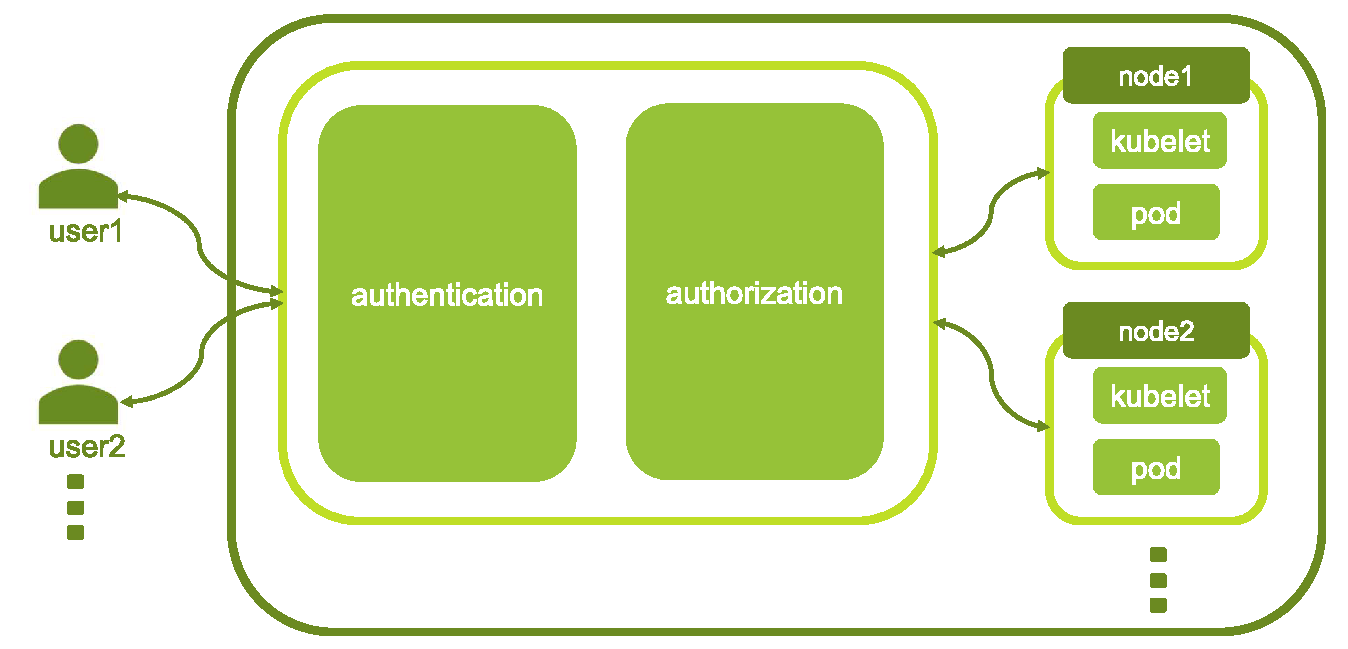
\includegraphics[width=0.86 \linewidth]{Thesis/Figures/Slide47.jpg}
\caption{\label{fig:Keycloak client}Creating Client in Keycloak}
\end{figure}

\clearpage

\textbf{Configure Root, Web and Admin URL}

When configuring a client in Keycloak, you need to set several URLs, including the Root URL, Web Origins and Admin URL as shown in \autoref{fig:Keycloak url}. The Root URL should be set to the base URL of your application, which Keycloak will use for redirects during authentication. The Web Origins field specifies allowed domains, ensuring that only the specified origins can interact with Keycloak from the browser. The Admin URL is used by Keycloak to send administrative actions, such as session invalidation, to the client. By setting all these URLs to the host name of your application, you establish a secure connection between Keycloak and your application for both frontend interaction and backend administration. \cite{keycloak_doc}

\begin{figure}[h]
\centering
\includegraphics[width=0.75 \linewidth]{Thesis/Figures/Slide51.jpg}
\caption{\label{fig:Keycloak url}Configure Root, Web and Admin URL}
\end{figure}

\textbf{Configure Client Secret, Roles and Users within Keycloak}

A client secret was generated for the ArgoCD client, ensuring that only authorized services can authenticate with Keycloak as shown in \autoref{fig:client secret}. This client secret acts as a secure credential that is required whenever ArgoCD requests authentication tokens from Keycloak, reinforcing the security of the integration. \cite{keycloak_doc}

\begin{figure}[h]
\centering
\includegraphics[width=0.7 \linewidth]{Thesis/Figures/Slide50.jpg}
\caption{\label{fig:client secret}Generating Client Secret in Keycloak}
\end{figure}

In order to implement fine-grained access control, roles have been defined within the Keycloak realm. These roles, such as admin, developer and viewer, encapsulate different levels of permissions, allowing for precise control over what users can do within ArgoCD. Assigning roles to users streamlines permission management and increases security by centralizing control within Keycloak. Finally, users were created and assigned the appropriate roles within Keycloak as shown in \autoref{fig:Keycloak user}. These users are the actual identities that will interact with ArgoCD and their roles determine their permissions, ensuring that access is tightly regulated based on organizational policies. \cite{keycloak_doc}


\begin{figure}[h]
\centering
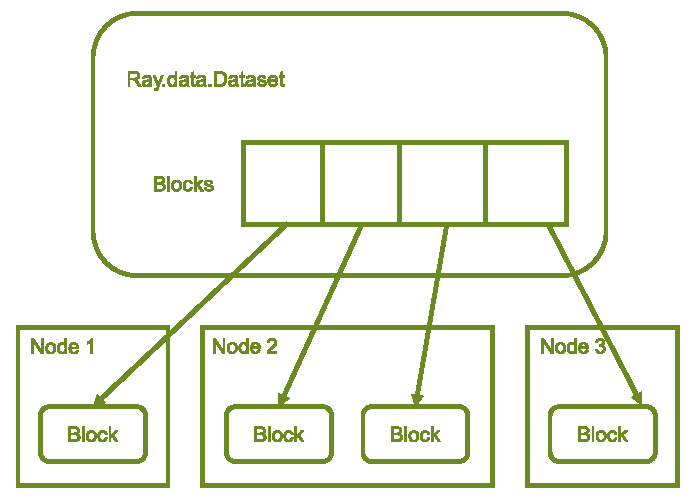
\includegraphics[width=0.8 \linewidth]{Thesis/Figures/Slide52.jpg}
\caption{\label{fig:Keycloak user}Creating User in Keycloak}
\end{figure}


\subsection{ArgoCD Configuration}

Configuring ArgoCD to use Keycloak as its OIDC provider involves several critical steps to ensure seamless authentication and secure integration between the two systems. The configuration focuses on modifying the ConfigMap and Secret within the Kubernetes cluster where ArgoCD is deployed, enabling it to authenticate users via Keycloak using the OIDC protocol for secure identity management and streamlined access. \cite{argocd_docs}


\textbf{Configuring ArgoCD to Use Keycloak as OIDC Provider}

To integrate Keycloak with ArgoCD, the first step is to configure client secret in ArgoCD to recognize Keycloak as its external identity provider using the client secret generated in Keycloak in the previous section. This process involves storing the client secret in the \texttt{argocd-secret}, which is the main secret used by ArgoCD for configuration. Begin by encoding the Keycloak client secret in base64 format then you need to edit the \texttt{argocd-secret} to include the base64 encoded client secret. This secret will be stored under a new key called \texttt{oidc.keycloak.clientSecret} as shown in code snippet \autoref{listingsnippet:5}. This modification allows ArgoCD to securely communicate with Keycloak as an external identity provider. \cite{argocd_docs}


\listingsnippet{Client Secret \cite{argocd_docs}}{

\vspace{0.3cm}

\hspace{0.25cm}\texttt{apiVersion: v1}

\hspace{0.25cm}\texttt{kind: Secret}

\hspace{0.25cm}\texttt{metadata:}

\hspace{0.5cm}\texttt{name: ArgoCD-secret}

\hspace{0.25cm}\texttt{data:}

\hspace{0.5cm}...

\hspace{0.5cm}\texttt{oidc.keycloak.clientSecret: <base64-encoded-client-secret>}

\hspace{0.5cm}...

\vspace{0.3cm}
}

To complete the integration of Keycloak with ArgoCD, the next step is to configure the ArgoCD ConfigMap to include the OIDC configuration that enables Keycloak authentication. In addition, we will set up access policies in ArgoCD to define roles for users authenticated by Keycloak. After updating the \texttt{argocd-cm} ConfigMap, the ConfigMap should look like code snippet \autoref{listingsnippet:6}. \cite{argocd_docs}

\listingsnippet{Configuring ConfigMap \cite{argocd_docs}}{

\vspace{0.3cm}

\hspace{0.25cm}\texttt{apiVersion: v1}

\hspace{0.25cm}\texttt{kind: ConfigMap}

\hspace{0.25cm}\texttt{metadata:}

\hspace{0.75cm}\texttt{name: argocd-cm}

\hspace{0.25cm}\texttt{data:}

\hspace{0.75cm}\texttt{oidc.config:}

\hspace{1.5cm}\texttt{name: keycloak}

\vspace{0.1cm}
  
\hspace{1.5cm}\texttt{issuer: http://192.168.49.2:30965/realms/argocd}

\vspace{0.1cm}
    
\hspace{1.5cm}\texttt{clientID: ArgoCD}

\vspace{0.1cm}
    
\hspace{1.5cm}\texttt{clientSecret: oidc.keycloak.clientSecret}

\vspace{0.1cm}
    
\hspace{1.5cm}\texttt{requestedScopes: ["openid", "profile", "email", "groups"]}

\vspace{0.1cm}
  
\hspace{0.75cm}\texttt{url: https://127.0.0.1:8080}

  \vspace{0.3cm}
}

In OIDC configuration it is required to define Issuer URL, ClientID, Client Secret and Scope. In which \texttt{issuer} URL is the endpoint of the Keycloak realm that ArgoCD will use to authenticate users. The \texttt{issuer} field must point to the Keycloak realm. The \texttt{clientID} corresponds to the client configured in Keycloak, which represents ArgoCD. The \texttt{clientSecret} is securely stored and used to authenticate the OIDC requests between ArgoCD and keycloak.
The \texttt{requestedScopes} field defines the permissions that ArgoCD requests from Keycloak, including standard OIDC scopes like \texttt{openid}, \texttt{profile}, \texttt{email} and \texttt{groups}. These scopes allow ArgoCD to obtain necessary user information and group memberships, which are then mapped to ArgoCD roles. \cite{argocd_docs}

\clearpage

After updating the ConfigMap with the OIDC configuration, it is essential to apply the changes to the Kubernetes cluster to activate the new settings \cite{argocd_docs}. Following the restart, users will see a \autoref{fig:login via keycloak} button on the ArgoCD landing page, indicating the successful integration of Keycloak as the identity provider for ArgoCD \cite{argocd_docs}. This button allows users to start the authentication process through Keycloak, enabling secure and centralized access control for ArgoCD \cite{argocd_docs}. When users attempt to log into ArgoCD, they will be redirected to the Keycloak login page to authenticate using their Keycloak credentials \cite{keycloak_doc}. After successful authentication, Keycloak redirects users back to ArgoCD, where authorization is managed based on the roles and claims provided by Keycloak \cite{keycloak_doc}.

\begin{figure}[h]
\centering
\includegraphics[width=1 \linewidth]{Thesis/Figures/Slide49.jpg}
\caption{\label{fig:login via keycloak}ArgoCD Login Via Keycloak}
\end{figure}

\subsection{Testing the Integration}

Having successfully configured ArgoCD to use Keycloak for SSO using OIDC protocol, the next step is to test the integration by logging into ArgoCD using Keycloak authentication. To begin testing, users will navigate to the ArgoCD web interface. On reaching the login page, they should now see an option to log in via Keycloak, indicating that the integration is active. Selecting the \texttt{Login via Keycloak} button will take users to the Keycloak authentication page where they enter their credentials. Once authenticated, Keycloak redirects the user back to ArgoCD, which processes the login and grants access based on the users roles and permissions as defined in Keycloak. A successful login indicates that the integration is working as expected and that all configurations between ArgoCD and Keycloak are correctly aligned.

\clearpage

\subsection{Challenges and Solutions}

During the integration process, several challenges arise that impact the functionality of the authentication system. One common issue is mismatched configurations between ArgoCD and Keycloak, particularly in the OIDC settings such as client ID, secret and redirect URIs. Ensuring that these configurations match exactly in both Keycloak and ArgoCD is crucial to avoiding authentication errors \cite{oauth_oidc_intro}. This issue is resolved by carefully reviewing the OIDC configuration in both platforms and ensuring they align with each other \cite{keycloak_doc}. Another challenge often encountered involves SSL/TLS certificates. ArgoCD and Keycloak both rely on secure HTTPS connections and any misconfiguration in SSL/TLS settings can result in failed connections between the two services. This problem can manifest as errors during the redirect process or outright failures to establish a secure session \cite{Kubernetes_doc}. The solution typically involves ensuring that valid SSL/TLS certificates are installed and properly configured in both Keycloak and ArgoCD, along with verifying that the correct certificate authorities are trusted by both systems \cite{argocd_docs}.

\section{Implementation of Authorization with Role-Based Access Control}

The implementation of RBAC in a Kubernetes cluster is critical to manage and secure access to resources. It provides a mechanism to define roles and assign permissions to users or groups using those roles. This approach is crucial in a multi-tenant environment where different users and applications require varying levels of access. By implementing RBAC, the cluster can enforce the principle of least privilege ensuring that users and services have only the permissions they need to perform their functions, thus reducing the risk of accidental or malicious actions. In Kubernetes RBAC is a built-in authorization mechanism that controls access to the API server and its resources. It uses four main concepts Roles, ClusterRoles, RoleBindings and ClusterRoleBindings. \cite{Kubernetes_doc}

\textbf{Roles and ClusterRoles} 

A Role and ClusterRole define a set of permissions where a Role is namespace scoped and ClusterRole is cluster-scoped. These permissions define which operations like Get, List, Create or Delete is allowed on certain resources such as Pods, Services, or Deployments. \cite{Kubernetes_doc}

\textbf{RoleBindings and ClusterRoleBindings} 

RoleBindings and ClusterRoleBindings are used to assign Roles or ClusterRoles to users or groups. A RoleBinding assigns a Role to a user within a specific namespace, while a ClusterRoleBinding assigns a ClusterRole to a user across the entire cluster. This separation of roles and bindings provides flexibility in how permissions are managed and assigned, allowing administrators to apply broad or narrow access controls as needed. Implementing RBAC in a Kubernetes cluster typically involves defining these roles and bindings in yet another markup language \abk{YAML}{Yet Another Markup Language} manifests, which are then applied to the cluster. For example, an administrator might create a role that allows read-only access to pods within a specific namespace and then bind that role to a group of developers. This ensures that the developers can view the pods but cannot modify or delete them, aligning their access level with their responsibilities. The configuration and management of RBAC are supported by tools like \texttt{kubectl}, which allows administrators to define and apply roles and bindings through command line operations. Additionally, RBAC policies can be dynamically updated as organizational needs evolve, ensuring that access controls remain aligned with the current security posture. \cite{Kubernetes_doc}

\subsection{Creating Roles and RoleBindings}

In RBAC system roles are created to assign permissions inside a namespace, as well as RoleBinding which is used to bind roles to users. Roles determine a given set of rights that outlines the kind of operations permitted on a set of objects in a namespace. For example, a Role might grant permissions to manage pods, services and deployments. This granularity ensures that users or service accounts have precise access based on their responsibilities. To define a Role, a YAML manifest is used, code snippet \autoref{listingsnippet:7} shows configuration for a example role named \texttt{developer-role}. \cite{Kubernetes_doc}

\listingsnippet{Role Configuration \cite{Kubernetes_doc}}{

\vspace{0.3cm}

\hspace{0.25cm}\texttt{apiVersion: rbac.authorization.k8s.io/v1}

\hspace{0.25cm}\texttt{kind: Role}

\hspace{0.25cm}\texttt{metadata:}

\hspace{0.75cm}\texttt{name: developer-role}

\hspace{0.75cm}\texttt{namespace: development}

\hspace{0.25cm}\texttt{rules:}

\hspace{0.25cm}\texttt{- apiGroups: [""]}

\hspace{0.75cm}\texttt{resources: ["pods", "services", "deployments"]}

\hspace{0.75cm}\texttt{verbs: ["get", "list", "create", "update", "delete"]}

\vspace{0.3cm}

}

Above YAML configuration grants permissions to manage pods, services and deployments within the \texttt{development} namespace. The \texttt{verbs} field specifies the actions allowed like get, list, create, update and delete. RoleBindings link the defined role to specific users, groups or service accounts within the namespace. This binding ensures that only the specified entities can perform the actions defined in the Role. For instance, code snippet \autoref{listingsnippet:8} shows YAML manifest to creates a RoleBinding that assign the \texttt{developer-role} to a user named \texttt{alice}. This RoleBinding guarantees that the user \texttt{alice} is granted the permissions defined in the \texttt{developer-role} for the \texttt{development} namespace. \cite{Kubernetes_doc} 

\listingsnippet{RoleBinding Configuration \cite{Kubernetes_doc}}{

\vspace{0.3cm}

\hspace{0.25cm}\texttt{apiVersion: rbac.authorization.k8s.io/v1}

\hspace{0.25cm}\texttt{kind: RoleBinding}

\hspace{0.25cm}\texttt{metadata:}

\hspace{0.75cm}\texttt{name: developer-role-binding}
  
\hspace{0.75cm}\texttt{namespace: development}
  
\hspace{0.25cm}\texttt{subjects:}

\hspace{0.25cm}\texttt{- kind: User}

\hspace{0.75cm}\texttt{name: alice}
  
\hspace{0.75cm}\texttt{apiGroup: rbac.authorization.k8s.io}

\hspace{0.25cm}\texttt{roleRef:}

\hspace{0.75cm}\texttt{kind: Role}
  
\hspace{0.75cm}\texttt{name: developer-role}
  
\hspace{0.75cm}\texttt{apiGroup: rbac.authorization.k8s.io}

\vspace{0.3cm}
}



\subsection{Creating ClusterRoles and ClusterRoleBindings}

ClusterRoles are used to define permissions that span across the entire Kubernetes cluster or across multiple namespaces. Unlike Roles, which are namespace scoped, ClusterRoles are cluster-scoped and are used for tasks that require broader access. Code snippet \autoref{listingsnippet:9} shows YAML configuration for a ClusterRole. \cite{Kubernetes_doc}


\listingsnippet{ClusterRole Configuration \cite{Kubernetes_doc}}{
\vspace{0.3cm}

\hspace{0.25cm}\texttt{apiVersion: rbac.authorization.k8s.io/v1}

\hspace{0.25cm}\texttt{kind: ClusterRole}

\hspace{0.25cm}\texttt{metadata:}

\hspace{0.75cm}\texttt{name: cluster-admin}

\hspace{0.25cm}\texttt{rules:}

\hspace{0.25cm}\texttt{- apiGroups: [""]}

\hspace{0.75cm}\texttt{resources: ["pods", "services", "deployments", "nodes"]}

\hspace{0.75cm}\texttt{verbs: ["get", "list", "create", "update", "delete"]}
\vspace{0.3cm}
}

The \texttt{cluster-admin} ClusterRole grants permissions to manage pods, services, deployments and nodes across the entire cluster . This role is essential for administrative functions that require cluster-wide access. ClusterRoleBindings bind ClusterRoles to users, groups, or service accounts, granting them the defined permissions across all namespaces. Code snippet \autoref{listingsnippet:10} shows the following YAML manifest creates a ClusterRoleBinding that assigns the \texttt{cluster-admin} ClusterRole to a user named \texttt{admin-user}. \cite{Kubernetes_doc}

\listingsnippet{ClusterRoleBinding Configuration \cite{Kubernetes_doc}}{
\vspace{0.3cm}

\hspace{0.25cm}\texttt{apiVersion: rbac.authorization.k8s.io/v1}

\hspace{0.25cm}\texttt{kind: ClusterRoleBinding}

\hspace{0.25cm}\texttt{metadata:}

\hspace{0.75cm}\texttt{name: cluster-admin-binding}

\hspace{0.25cm}\texttt{subjects:}

\hspace{0.25cm}\texttt{- kind: User}

\hspace{0.75cm}\texttt{name: admin-user}

\hspace{0.75cm}\texttt{apiGroup: rbac.authorization.k8s.io}
  
\hspace{0.25cm}\texttt{roleRef:}

\hspace{0.75cm}\texttt{kind: ClusterRole}
  
\hspace{0.75cm}\texttt{name: cluster-admin}
  
\hspace{0.75cm}\texttt{apiGroup: rbac.authorization.k8s.io}
\vspace{0.3cm}
}

This ClusterRoleBinding ensures that the user \texttt{admin-user} has administrative privileges across the entire Kubernetes cluster . By configuring these roles and bindings, administrators can effectively manage permissions, ensuring appropriate access levels while maintaining the security and integrity of the cluster. \cite{Kubernetes_doc}

\subsection{Automating Role-Based Access Control Authorization}

The automation of process of RBAC authorization consists of two steps first a private key and certificate signing request \abk{CSR}{Certificate Signing Request} is generated for the user and then in next step role and role binding or cluster role or cluster role binding is generated by automation script. \cite{Kubernetes_doc}

\textbf{User Creation}

The process of user creation begins with the generation of a private key and CSR specific to the user, which is essential for secure authentication. This CSR is then submitted to Kubernetes as a CSR object, which allows the user to be recognized as a system authenticated entity. The automation system handles the approval of the CSR, simulating the role of an administrator and retrieves the signed certificate upon approval. Once the certificate is issued, the system automatically configures the \texttt{kubeconfig} file by setting the users credentials and creating a new context that associates the user with the designated cluster and namespace. \cite{Kubernetes_doc}

\textbf{Creating Roles and Assigning it to Users}

The automated process of creating roles and binding them to users in a specified namespace, thereby streamlining access control within the cluster. The process begins by checking for the existence of the specified Role and RoleBinding to avoid duplication and ensure accurate configuration. It then automatically creates a Role with specific permissions, allowing the designated user to perform actions such as \texttt{get}, \texttt{list} and \texttt{watch} pods within the specified namespace. Once the role has been defined, the process creates a RoleBinding that associates the role with the user, thereby granting the appropriate permissions defined in the role. This automated approach ensures that access is consistently managed according to predefined security policies, reduces the potential for manual errors and facilitates efficient user management within Kubernetes environments, improving security and operational efficiency. This configuration allows the user to interact with the cluster in a secure manner and with the appropriate permissions as defined by the RBAC policies. The automated process significantly reduces manual intervention, ensures consistent user setup, minimises errors and increases the overall efficiency of managing access control in Kubernetes environments. \cite{Kubernetes_doc}

\subsection{Testing Role-Based Access Control}

Testing RBAC in Kubernetes involves verifying that users and service accounts can access only the resources and perform the actions they are authorized for, based on their assigned roles and role bindings. In this research different roles with varying permissions are defined and then assign these roles to different users or groups. For example, a user with an \texttt{admin} role should have full access to all resources, while a \texttt{developer} role might only have permissions to manage pods and services within a specific namespace. To validate the configuration, test were conducted by logging in as different users and attempting to perform operations that should be either allowed or denied according to their roles. For instance, a user assigned the \texttt{viewer} role should be able to view resources but should not be able to create or delete them, that show only the user with specific permissions and access levels, interact with the resources as intended. \cite{Kubernetes_doc}


\subsection{Challenges and Solutions}

Implementing RBAC can present several challenges, like overly permissive roles in which, one common issue is assigning overly broad permissions to roles, which might grant users more access than necessary. For example, if a \texttt{developer} role is mistakenly given \texttt{delete} permissions for all resources, it could lead to accidental or malicious deletion of critical resources. To mitigate this, carefully review and test role definitions and apply the principle of least privilege, granting only the permissions necessary for each role. Another challenge is creating incorrect or misconfigured RoleBindings and ClusterRoleBindings. For instance, binding a ClusterRole that has extensive permissions to a user who only needs limited access can pose a security risk. \cite{Kubernetes_doc}

\section{Implementation of Scalable Architectures}

Providing a scalable architecture for AI models is critical to meet the growing computational demands associated with modern ML workloads. In this implementation, Ray was chosen for its ability to handle distributed workloads making it an ideal choice for running AI models that require significant computational resources \cite{ray_doc}. To ensure both performance and cost efficiency the key objective was to create a system that could automatically adjust resources based on the workload. The deployment process began with the creation of a Kubernetes cluster which serves as the foundation for container orchestration and management \cite{Kubernetes_doc}. Kubernetes was chosen for its scalability features and support for managing containerised applications in production environments \cite{r4}. The cluster was created using Kind, which makes it easy to create a Kubernetes environment using Docker containers \cite{kind2021}. Once the Kubernetes cluster was in place then the next step was to deploy Ray on top of it. The Ray architecture allows tasks to scale seamlessly across multiple nodes, ensuring efficient use of resources \cite{ray_doc}. The Ray cluster was deployed using KubeRay, an operator that simplifies the management of Ray clusters on Kubernetes \cite{ray_doc}. KubeRay automates the provisioning, scaling and management of Ray clusters, which was essential for maintaining a stable and scalable environment \cite{burns2021designing}. To enable autoscaling, the Ray cluster was configured with autoscaling capabilities using KubeRay \cite{ray_doc}. Autoscaling is a critical feature that dynamically adjusts the number of worker nodes in the Ray cluster based on workload demands \cite{Kubernetes_doc}. This ensures that the cluster scales up when demand for compute resources is high, and scales down when demand decreases, optimising both performance and cost \cite{liu2019scalable}. The autoscaling configuration was defined in a YAML file, specifying the minimum and maximum number of worker nodes and the conditions under which scaling should occur \cite{ray_doc}. In addition to autoscaling, the Ray cluster was configured to support GPU access, which is essential for AI workloads involving large models \cite{wong2021gpu}. GPU support was enabled by specifying GPU resources in the Ray cluster configuration, allowing the cluster to use hardware accelerators for faster computation \cite{nvidia_gpu_operator}. This configuration was particularly important for training large neural networks, which require significant computing power \cite{goodfellow2016deep}. The final step was to validate the deployment by running AI model training tasks on the Ray cluster. The tasks were distributed across multiple nodes, with the autoscaler dynamically adjusting resources as needed \cite{spark_unified_engine}. This deployment successfully demonstrated the ability to scale AI model execution in a production like environment, meeting the objective of creating a scalable and efficient architecture for AI workloads \cite{dean2008mapreduce}.

\subsection{Ray on Kubernetes}

Ray cluster utilize Kubernetes orchestration capabilities to manage distributed computing tasks efficiently. Deploying Ray in a Kubernetes environment enables the scaling and management of complex AI workflows by leveraging Kubernetes features such as resource management, fault tolerance and automated scaling. This setup integrates distributed components of Ray, like Ray Core, Ray Data, Ray Train and Ray Tune within Kubernetes to handle large-scale ML tasks effectively. The synergy between Ray distributed computing framework and Kubernetes container orchestration facilitates a scalable and resilient infrastructure for AI applications \cite{moritz}. KubeRay extends this integration by providing an operator specifically designed to manage Ray clusters within Kubernetes. The KubeRay operator automates the deployment, scaling and management of Ray resources, each Ray cluster consisting of a head node and a collection of worker nodes, as shown in \autoref{fig:Ray on Kubernetes}. Ray clusters adapt dynamic Kubernetes environment by handling tasks such as autoscaling and GPU resource management, which provides support for adding or removing pods as needed. Thus, Kubernetes provides the basic orchestration, KubeRay complements it by streamlining the management of Ray distributed tasks, ultimately enabling efficient and scalable AI workload management. \cite{ray_doc}

\clearpage

\begin{figure}[h]
\centering
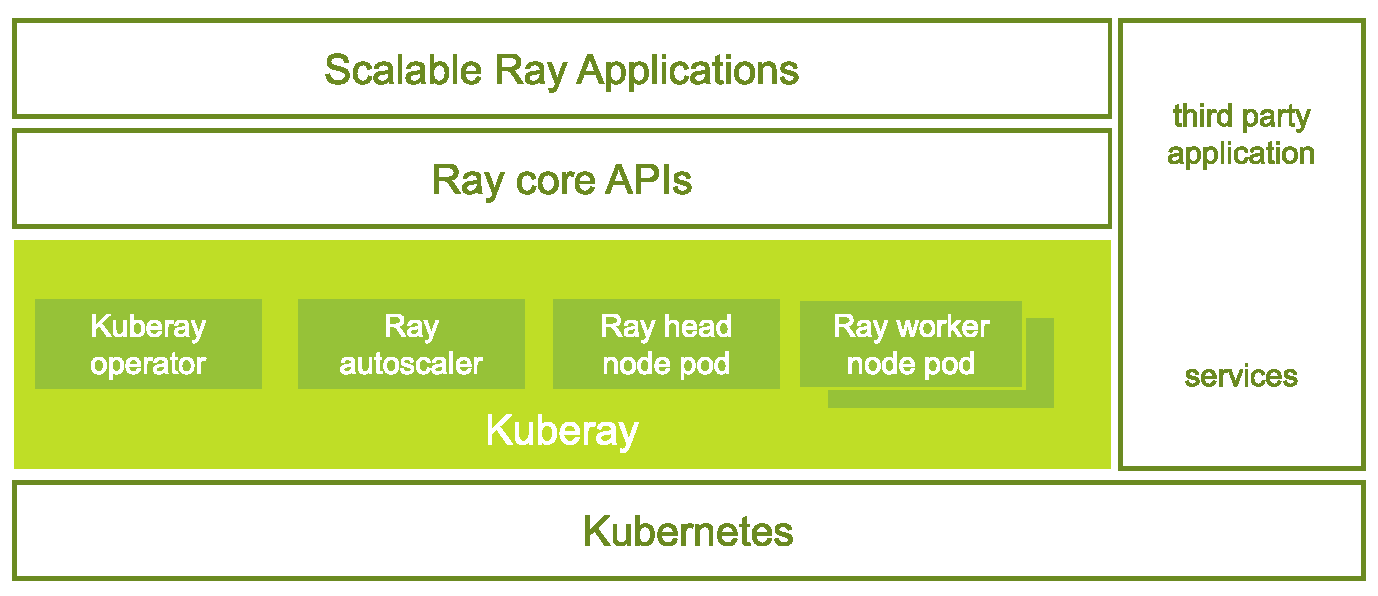
\includegraphics[width=1 \linewidth]{Thesis/Figures/Slide54.pdf}
\caption{\label{fig:Ray on Kubernetes}Ray on Kubernetes \cite{ray_doc}}
\end{figure}



\subsection{Setup Ray Cluster}

Setting up a Ray cluster within a Kubernetes environment requires several dependencies to ensure seamless integration and functionality. The initial step involves installing essential software, including Kubernetes and its associated tools like \texttt{kubectl}, which is necessary for managing the Kubernetes environment \cite{Kubernetes_doc}. Additionally, Docker is required to containerize the Ray components, while Helm is used to manage Kubernetes applications through Helm charts \cite{helm_docs}. For local Kubernetes cluster setup, tools such as kind can be utilized to create a lightweight, local cluster for development and testing purposes \cite{kind2021}. These dependencies are fundamental for creating a robust and scalable Ray cluster that can efficiently handle distributed computing tasks. The installation process for Ray involves deploying core Ray components and configuring them for Kubernetes integration. Start by installing the Ray core component, which forms the backbone of the Ray distributed computing framework. This is followed by the installation of Ray data for handling large datasets, Ray train for training ML models and Ray tune for hyperparameter tuning \cite{ray_doc}. Additional methods such as Ray actor and Ray job facilitate the management and execution of tasks and jobs within the Ray cluster \cite{ray_doc}. To integrate Ray with Kubernetes, KubeRay is deployed, which includes setting up the KubeRay operator. This operator manages the lifecycle of Ray clusters within Kubernetes \cite{ray_doc}. The configuration involves updating Ray autoscaler settings and applying them through Kubernetes manifests, ensuring that the cluster scales dynamically based on workload demands \cite{ray_doc}. By following these steps, the Ray cluster is set up to leverage Kubernetes orchestration capabilities, providing a scalable and efficient environment for running AI and ML workloads.

\subsection{KubeRay Autoscaling}

KubeRay uses Kubernetes HPA for dynamic resource management in Ray clusters. This integration ensures that Ray clusters can automatically adjust their size based on the workload according to the ratio of the current metric value to optimise resource utilization and maintain cluster performance. \cite{Kubernetes_doc}

\textbf{Horizontal Pod Autoscaling}

HPA is used to scale number of worker pods in a deployment based on observed metrics such as CPU utilization or any custom metrics \cite{Kubernetes_doc}. For Ray clusters, configuring HPA allows the number of Ray worker pods to automatically scale up or down in response to automatically adjust the load and ensuring that resources are allocated and used efficiently \cite{Kubernetes_doc}. The configuration of HPA required to achieve autoscaling is shown in code snippet \autoref{listingsnippet:11}.

\listingsnippet{HPA Configuration within Ray  \cite{ray_doc}}{

\vspace{0.3cm}

\hspace{0.25cm}\texttt{apiVersion: autoscaling/v2beta2}

\hspace{0.25cm}\texttt{kind: HorizontalPodAutoscaler}

\hspace{0.25cm}\texttt{metadata:}

\hspace{0.75cm}\texttt{name: ray-worker-hpa}

\hspace{0.75cm}\texttt{namespace: default}

\hspace{0.25cm}\texttt{spec:}

\hspace{0.75cm}\texttt{scaleTargetRef:}

\hspace{1.5cm}\texttt{apiVersion: apps/v1}

\hspace{1.5cm}\texttt{kind: Deployment}

\hspace{1.5cm}\texttt{name: ray-worker}

\hspace{0.75cm}\texttt{minReplicas: 2}

\hspace{0.75cm}\texttt{maxReplicas: 10}

\hspace{0.75cm}\texttt{metrics:}

\hspace{0.75cm}\texttt{- type: Resource}
    
\hspace{1.5cm}\texttt{resource:}
    
\hspace{2cm}\texttt{name: cpu}

\hspace{2cm}\texttt{target:}

\hspace{2.5cm}\texttt{type: Utilization}

\hspace{2.5cm}\texttt{averageUtilization: 50}

\vspace{0.3cm}
}


This configuration ensures that the number of Ray worker pods is adjusted between 2 and 10 based on the average CPU utilization. By setting these parameters, the HPA maintains an optimal number of pods to handle varying workloads efficiently. \cite{Kubernetes_doc}

\textbf{Detached and Terminate Detached Actors}

Ray actor model supports detached and terminated detached actors, which are essential for managing long running and stateful tasks within a Ray cluster. Detached and terminate detached actors continue to operate independently of the cluster lifecycle, which allows for continuity in ongoing computations even during scaling events. Detached actors are designed to persist across scaling or restart events. They continue executing their tasks and maintaining their state, which is crucial for computations that require continuity. To manage resources effectively, detached actors can be terminated when they are no longer needed. This ensures that resources are reclaimed and utilized efficiently during scaling events. \cite{ray_doc}

\clearpage

\textbf{Hyperparameter Tuning Trials with Ray Tune}

In this phase of the implementation, the autoscaling process was tested by varying the number of hyperparameter tuning trials. As the volume of trials increased, the computational load on the Ray cluster also increased, thereby necessitating the scaling of the worker pods. The underlying principle involves scaling the number of Ray worker pods based on the demands of the hyperparameter tuning process. The \texttt{tune.run()} function configuration in Kubernetes, as shown in the code snippet \autoref{listingsnippet:12}, was used to tune hyperparameters, initiated multiple hyperparameter search trials, which impacted the workload and triggered autoscaling to manage the increased demand. The HPA monitored CPU utilization and adjusted the number of pods accordingly, ensuring that the cluster could handle the computational load efficiently. \cite{ray_doc}

\listingsnippet{Hyperparameter Tuning Trials with Ray Tune \cite{ray_doc}}{
\vspace{0.3cm}

\hspace{0.25cm}\texttt{\# Configure Ray Tune}

\vspace{0.3cm}

\hspace{0.25cm}\texttt{analysis = tune.run(}

\vspace{0.3cm}

\hspace{0.75cm}\texttt{train-model,}

\hspace{0.75cm}\texttt{config=search-space,}

\hspace{0.75cm}\texttt{numsamples=10,}

\hspace{0.75cm}\texttt{metric="metric",}

\hspace{0.75cm}\texttt{mode="max",}

\hspace{0.75cm}\texttt{resources-per-trial={"cpu": 1},}

\hspace{0.75cm}\texttt{verbose=1,}

\vspace{0.3cm}

\texttt{)}
    
\vspace{0.3cm}  
}



\subsection{Ray cluster Autoscaling Workflow}

Enabling a scalable architecture with Ray involves several installation and configuration steps. Including creating a cluster, deploying the KubeRay operator, enabling autoscaling and installing dependencies. The workflow is designed to automate the process of configuring scalable Ray cluster on Kubernetes using Kind and KubeRay. The process starts with the creation of a custom Docker image initialize with the official Ray image and additional dependencies required by the model such as scikit-learn are added as shown in code snippet \autoref{listingsnippet:13}. This Docker image is automatically built from a Docker file and pushed to a Docker registry for future use. In next step a Kubernetes cluster is created using Kind. Once the cluster is created, the workflow then deploys the KubeRay operator which manages Ray clusters within Kubernetes. The KubeRay Helm repository is then added and operator is deployed in a dedicated namespace to ensure efficient cluster management and scaling. After setting up the operator script updates Ray autoscaler configuration to use the custom Docker image created in the first step. The updated configuration makes sure that all the necessary dependencies is installed using Docker image. Then autoscaling configuration is applied to deploy a Ray cluster with autoscaling enabled. This allows the cluster to dynamically scale its resources with all the dependencies installed. Finally, the script monitors the deployment by continuously checking the pods in the specified namespace and verifying that everything is running as expected. This automated workflow allows ML engineers to efficiently set up a scalable computing environment using Ray clusters in Kubernetes simplifying resource management and automating scaling for computational tasks that require dynamic resource allocation.

\listingsnippet{Docker Images to Install Dependencies}{

\vspace{0.3cm}


\hspace{0.25cm}\texttt{\# Start from the official Ray image}

\hspace{0.25cm}\texttt{FROM rayproject/ray:2.9.0}

\vspace{0.3cm}

\hspace{0.25cm}\texttt{\# Install scikit-learn and any other dependencies you need}

\hspace{0.25cm}\texttt{RUN pip install scikit-learn}

\vspace{0.3cm}
}

\subsection{Installing Dependencies to Resources}



Installing dependencies in a containerized environment is essential to ensure that the application has all the required libraries and tools to function correctly. These dependencies, whether they are specific programming language libraries, system tools, or other runtime utilities, are vital for running the code within the container, without them the application might not start or could encounter errors during execution, leading to service disruptions. Properly managing and installing these dependencies not only ensures that the application works as expected but also enhances its portability and consistency across different environments. This becomes particularly important in dynamic environments, such as distributed computing, where resources are scaled up or down frequently and ensuring that the required dependencies are always available to maintain performance and functionality. Two primary methods to handle dependency installation in distributed environments is implemented in this research. \cite{Kubernetes_doc, loft2024adding}

\begin{itemize}
    \item Container image method
    \item Container lifecycle hooks
\end{itemize}

\textbf{Container Image Method}

In container image method, dependencies can be managed efficiently by creating a Docker file that lists and installs all the necessary libraries, system tools and other utilities required by the application. This Docker file can include commands such as \texttt{RUN pip install} for Python libraries or \texttt{RUN apt-get install} for system dependencies, ensuring that the container image is built with everything the application needs to run. Once the image is built, it is used in the pod's YAML configuration to ensure that the container starts with all dependencies preinstalled as shown in code snippet \autoref{listingsnippet:14}. When Kubernetes scales the application using HPA, it automatically deploys new worker pods using this pre-configured image, ensuring all dependencies are already installed on all worker nodes. This approach not only ensures consistency across environments, but also speeds up the startup process for new pods by eliminating the need for additional installations at runtime. With this configuration, Kubernetes can efficiently scale resources while maintaining reliable, independent environment for all pods. \cite{Kubernetes_doc, loft2024adding}

\listingsnippet{Updated Pod Configuration using Docker Image \cite{Kubernetes_doc}}{

\vspace{0.3cm}
 
\hspace{0.25cm}\texttt{headGroupSpec:}

\hspace{0.75cm}\texttt{rayStartParams:}

\hspace{1.25cm}\texttt{num-cpus: "0"}

\hspace{0.75cm}\texttt{template:}

\hspace{1.25cm}\texttt{spec:}

\hspace{1.75cm}\texttt{containers:}

\hspace{1.75cm}\texttt{- image: my-custom-ray:2.9.0}

\hspace{2.25cm}\texttt{lifecycle:}

\hspace{2.75cm}\texttt{preStop:}

\hspace{3,25cm}\texttt{exec:}

\hspace{3.75cm}\texttt{command:}

\hspace{3.75cm}\texttt{- /bin/sh}

\hspace{3.75cm}\texttt{- -c}

\hspace{3.75cm}\texttt{- ray stop}

\vspace{0.3cm}
}

\textbf{Container Lifecycle Hooks}


Container lifecycle hook allows containers to execute specific code and installation processes triggered by events during its administrative lifecycle. These hooks provide flexibility in handling actions during the container lifecycle by allowing containers to be aware of specific events and execute code when triggered. PostStart and PreStop are the two primary hooks exposed to containers. The PostStart hook is executed immediately after a container is created, allowing custom code to be executed when the container starts. This can be useful for installing dependencies or performing other setup tasks that need to occur at the start of the container, but after the image has been initialised. The hook can be configured in the pod's YAML configuration, as shown in the code snippet \autoref{listingsnippet:15}. 

\listingsnippet{Update Pod Configuration using PostStart Hooks \cite{Kubernetes_doc}}{

\vspace{0.3cm}
 
\hspace{0.25cm}\texttt{headGroupSpec:}

\hspace{0.75cm}\texttt{rayStartParams:}

\hspace{1.25cm}\texttt{num-cpus: "0"}

\hspace{0.75cm}\texttt{template:}

\hspace{1.25cm}\texttt{spec:}

\hspace{1.75cm}\texttt{containers:}

\hspace{1.75cm}\texttt{- image: rayproject/ray:2.9.0}

\hspace{2.25cm}\texttt{lifecycle:}

\hspace{2.75cm}\texttt{postStop:}

\hspace{3,25cm}\texttt{exec:}

\hspace{3.75cm}\texttt{command: ["/bin/bash", "-c", "/bin/setup-head.sh"]}

\vspace{0.3cm}
}

The second hook, PreStop, is executed just before the container is destroyed, typically triggered by events such as API requests or resource contention. The PreStop hook allows containers to handle termination gracefully by performing specific shutdown procedures, such as saving state or closing connections, before the container is stopped. Like the PostStart hook, the container will eventually terminate within its grace period, regardless of the outcome of the handler. An example configuration of the PreStop hook is shown in the code snippet at \autoref{listingsnippet:16}.





\listingsnippet{Update Pod Configuration using PreStop Hooks \cite{Kubernetes_doc}}{

\vspace{0.3cm}
 
\hspace{0.25cm}\texttt{workerGroupSpec:}

\hspace{0.75cm}\texttt{rayStartParams:}

\hspace{1.25cm}\texttt{num-cpus: "0"}

\hspace{0.75cm}\texttt{template:}

\hspace{1.25cm}\texttt{spec:}

\hspace{1.75cm}\texttt{containers:}

\hspace{1.75cm}\texttt{- image: rayproject/ray:2.9.0}

\hspace{2.25cm}\texttt{lifecycle:}

\hspace{2.75cm}\texttt{preStop:}

\hspace{3,25cm}\texttt{exec:}

\hspace{3.75cm}\texttt{command: ["/bin/bash", "-c", "/bin/setup-head.sh"]}

\vspace{0.3cm}
}

\subsection{GPU Access in KubeRay}

Accessing GPU is critical to achieve high performance in computing related to ML and deep learning \abk{DL}{Deep Learning} workloads \cite{nvidia_gpus_ai_ml}. GPU enables fast processing of large datasets and complex AI models and provides high processing power \cite{nvidia_gpus_ai_ml}. In KubeRay enabling GPU access involves several steps. First Kubernetes nodes must be equipped with GPUs and the necessary NVIDIA drivers and container runtime must be installed \cite{Kubernetes_doc}. Kubernetes uses the NVIDIA device plugin to expose GPUs to pods which must be properly configured in the Ray cluster setup \cite{Kubernetes_doc}. The Ray cluster configuration file must include resource requirements and limits for GPUs in the worker pod definitions. For example, in the YAML configuration file for the Ray cluster, you would specify the number of GPUs required by setting \texttt{nvidia.com/gpu} in the \texttt{resources} section of the worker pod configuration. This ensures that the Ray tasks requiring GPU resources are scheduled on nodes where GPUs are available \cite{ray_doc}. Configuration shows in code snippet \autoref{listingsnippet:17}, where each Ray worker pod is configured to request a GPU. This setup allows the Ray cluster to efficiently utilize GPU resources, thereby accelerating the processing of tasks that benefit from parallel computing, such as neural network training. \cite{ray_doc}

\listingsnippet{Ray Cluster Configuration with GPU Request \cite{ray_doc}}{

\vspace{0.3cm}

\hspace{0.25cm}\texttt{apiVersion: ray.io/v1alpha1}

\hspace{0.25cm}\texttt{kind: RayCluster}

\hspace{0.25cm}\texttt{metadata:}

\hspace{0.75cm}\texttt{name: ray-cluster}

\hspace{0.25cm}\texttt{spec:}

\hspace{0.75cm}\texttt{workerGroupSpecs:}

\hspace{1.5cm}\texttt{- replicas: 2}

\hspace{2cm}\texttt{template:}

\hspace{2.5cm}\texttt{spec:}

\hspace{3cm}\texttt{containers:}

\hspace{3.5cm}\texttt{- name: ray-worker}

\hspace{4cm}\texttt{image: rayproject/ray-ml:latest}

\hspace{4cm}\texttt{resources:}

\hspace{4.5cm}\texttt{limits:}

\hspace{5cm}\texttt{nvidia.com/gpu: 1}

\hspace{4.5cm}\texttt{requests:}

\hspace{5cm}\texttt{nvidia.com/gpu: 1}

\vspace{0.3cm}

}
                  
Furthermore, KubeRay supports dynamic scaling of GPU resources, aligning with the broader autoscaling capabilities of Ray clusters. This means that as the demand for GPU intensive tasks increases, KubeRay can scale the number of GPU equipped worker pods accordingly, ensuring that computational resources match the workload requirements. \cite{ray_doc}








